% This is samplepaper.tex, a sample chapter demonstrating the
% LLNCS macro package for Springer Computer Science proceedings;
% Version 2.21 of 2022/01/12
%
\documentclass[runningheads]{llncs}
%
\usepackage[T1]{fontenc}
% T1 fonts will be used to generate the final print and online PDFs,
% so please use T1 fonts in your manuscript whenever possible.
% Other font encondings may result in incorrect characters.
%
\usepackage{graphicx}
% Used for displaying a sample figure. If possible, figure files should
% be included in EPS format.
%
% If you use the hyperref package, please uncomment the following two lines
% to display URLs in blue roman font according to Springer's eBook style:
%\usepackage{color}
%\renewcommand\UrlFont{\color{blue}\rmfamily}
%\urlstyle{rm}
%
\usepackage{listings}
\usepackage{xcolor} % Para poder usar colores

\lstset{
    language=HTML,
    basicstyle=\ttfamily\small,      % Fuente monoespaciada
    keywordstyle=\color{blue},       % Etiquetas en azul
    stringstyle=\color{orange},      % Texto entre comillas en naranja
    commentstyle=\color{gray},       % Comentarios en gris
    breaklines=true,                 % Ajustar líneas largas
    frame=single,                    % Pone el recuadro (cuadrado)
    numbers=left,                    % Números de línea a la izquierda
    numberstyle=\tiny\color{gray},   % Estilo de los números
    showstringspaces=false,          % No mostrar espacios marcados
}
\begin{document}
%
\title{Modulo 1: Avogadro Toast}
%
%\titlerunning{Abbreviated paper title}
% If the paper title is too long for the running head, you can set
% an abbreviated paper title here
%
\author{Lucia Salamone \and
Lucas Segura \and
Pilar Mujica\and
Sara Kemelmajer\and
Rocio Martinez\and
Caterina Dinnocenzo}
%
\authorrunning{L. Salamone}
% First names are abbreviated in the running head.
% If there are more than two authors, 'et al.' is used.
%
\institute{Universidad Nacional de Cuyo, Instituto de Ingenería Industrial POBOX 5502 %\and
%Springer Heidelberg, Tiergartenstr. 17, 69121 Heidelberg, Germany
\email{luchisalamone10@gmail.com}\\
\url{https://ingenieria.uncuyo.edu.ar/}} %\and
%ABC Institute, Rupert-Karls-University Heidelberg, Heidelberg, Germany\\
%\email{\{abc,lncs\}@uni-heidelberg.de}}
%
\maketitle              % typeset the header of the contribution
%
\begin{abstract}
Durante el Módulo 1 adquirimos las bases fundamentales para el trabajo colaborativo y la creación de contenidos digitales orientados a proyectos académicos y profesionales. En la primera clase comenzamos creando nuestras cuentas en GitHub, donde configuramos un repositorio personal y también un repositorio grupal. Organizamos los equipos de trabajo, definimos un nombre e identidad (incluyendo logo) y aprendimos a estructurar información mediante tablas e inserción de imágenes, además de crear páginas individuales en Markdown y vincularlas a la página del grupo.

En la segunda clase incorporamos herramientas complementarias como Google Colab, lo \cite{lopez2003latex}que nos permitió familiarizarnos con notebooks. También aprendimos a crear archivos HTML de forma manual y exploramos conceptos básicos de HTML siguiendo estándares W3C, aplicándolos en la construcción de una landing page simple.

En la tercera clase dimos \cite{sepulcre2024uso}el salto a la escritura académica con LaTeX mediante Overleaf. Creamos nuestras cuentas, exploramos su funcionamiento y seleccionamos plantillas. A partir de esto, comenzamos el desarrollo de nuestro currículum en LaTeX, enfocándonos en la estructura profesional y presentación formal.

En conjunto, el módulo nos brindó herramientas clave para el trabajo en equipo, el manejo de repositorios y la generación de contenido técnico estructurado.


\keywords{UNCuyo \and TyHM \and markuo language.}
\end{abstract}
%
%
%
\section{Uso básico de GitHub}
\subsection{A Subsection Sample}
Please note that the first paragraph of a section or subsection is
not indented. The first paragraph that follows a table, figure,
equation etc. does not need an indent, either.

Subsequent paragraphs, however, are indented.

\subsubsection{Sample Heading (Third Level)} Only two levels of
headings should be numbered. Lower level headings remain unnumbered;
they are formatted as run-in headings.

\paragraph{Sample Heading (Fourth Level)}
The contribution should contain no more than four levels of
headings. Table~\ref{tab1} gives a summary of all heading levels.
\section{Uso básico del lenguaje html}

\begin{lstlisting}[language=HTML]
<html>
<head>
<title>Mi primera pagina</title>
</head>
<body>
<h1>Mi primera pagina web</h1>
Esto es el cuerpo del texto.
<p>Esto es un parrafo</p>
<ul>
<li>Primero</li>
<li>Segundo</li>
<li>Tercero</li>
</ul>
</body>
</html>
\end{lstlisting}


\begin{table}
\caption{Table captions should be placed above the
tables.}\label{tab1}
\begin{tabular}{|l|l|l|}
\hline
Heading level &  Example & Font size and style\\
\hline
Title (centered) &  {\Large\bfseries Lecture Notes} & 14 point, bold\\
1st-level heading &  {\large\bfseries 1 Introduction} & 12 point, bold\\
2nd-level heading & {\bfseries 2.1 Printing Area} & 10 point, bold\\
3rd-level heading & {\bfseries Run-in Heading in Bold.} Text follows & 10 point, bold\\
4th-level heading & {\itshape Lowest Level Heading.} Text follows & 10 point, italic\\
\hline
\end{tabular}
\end{table}


\noindent Displayed equations are centered and set on a separate
line.
\begin{equation}
x + y = z
\end{equation}
Please try to avoid rasterized images for line-art diagrams and
schemas. Whenever possible, use vector graphics instead (see
Fig.~\ref{fig1}).

\begin{figure}
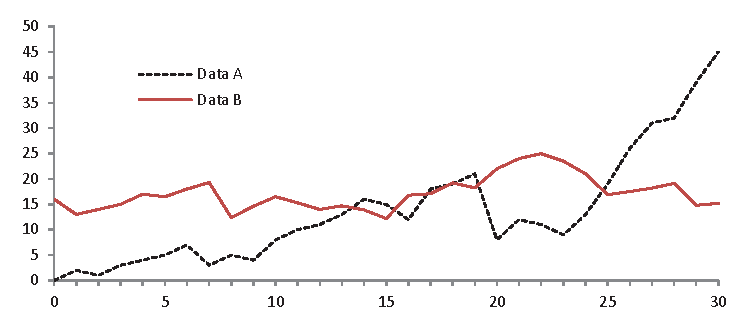
\includegraphics[width=\textwidth]{fig1.eps}
\caption{A figure caption is always placed below the illustration.
Please note that short captions are centered, while long ones are
justified by the macro package automatically.} \label{fig1}
\end{figure}

\begin{theorem}
This is a sample theorem. The run-in heading is set in bold, while
the following text appears in italics. Definitions, lemmas,
propositions, and corollaries are styled the same way.
\end{theorem}
%
% the environments 'definition', 'lemma', 'proposition', 'corollary',
% 'remark', and 'example' are defined in the LLNCS documentclass as well.
%
\begin{proof}
Proofs, examples, and remarks have the initial word in italics,
while the following text appears in normal font.
\end{proof}
For citations of references, we prefer the use of square brackets
and consecutive numbers. Citations using labels or the author/year
convention are also acceptable. The following bibliography provides
a sample reference list with entries for journal
articles~\cite{ref_article1}, an LNCS chapter~\cite{ref_lncs1}, a
book~\cite{ref_book1}, proceedings without editors~\cite{ref_proc1},
and a homepage~\cite{ref_url1}. Multiple citations are grouped
\cite{ref_article1,ref_lncs1,ref_book1},
\cite{ref_article1,ref_book1,ref_proc1,ref_url1}.

\begin{credits}
\subsubsection{\ackname} A bold run-in heading in small font size at the end of the paper is
used for general acknowledgments, for example: This study was funded
by X (grant number Y).

\subsubsection{\discintname}
It is now necessary to declare any competing interests or to specifically
state that the authors have no competing interests. Please place the
statement with a bold run-in heading in small font size beneath the
(optional) acknowledgments\footnote{If EquinOCS, our proceedings submission
system, is used, then the disclaimer can be provided directly in the system.},
for example: The authors have no competing interests to declare that are
relevant to the content of this article. Or: Author A has received research
grants from Company W. Author B has received a speaker honorarium from
Company X and owns stock in Company Y. Author C is a member of committee Z.
\end{credits}
%
% ---- Bibliography ----
%
% BibTeX users should specify bibliography style 'splncs04'.
% References will then be sorted and formatted in the correct style.
%
% \bibliographystyle{splncs04}
% \bibliography{mybibliography}
%
\bibliographystyle{splncs04} 
\bibliography{bibliografia} % <-- Aquí pones el nombre exacto de tu archivo sin el .bib
\end{document}